% !TEX root = ../rapport.tex
\newpage
\section{I2C kommunikation}
Til at kommunikere med de digitale komponenter, herunder vores udleveret accelerometer og gyroskop, anvendes den kommunikationsprotokol kaldet I2C eller TWI (”two-wire interface”). Navnet ”two-wire interface” kommer af, at hele kommunikationen foregår over kun 2 ledninger, men hvor der samtidig er mulighed for at kommunikere med mange komponenter.

\begin{figure}[ht]
    \centering
    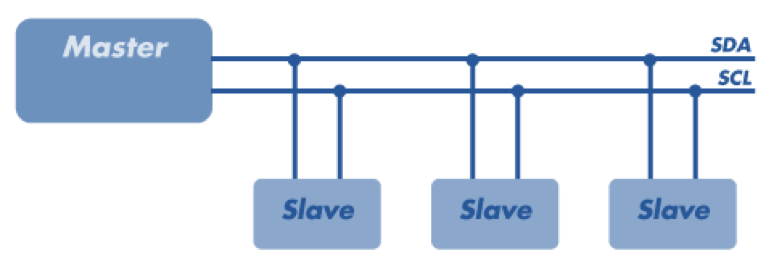
\includegraphics[width=0.8\textwidth]{kapitler/billeder/i2c-princip.png}
    \caption{Viser en skitse af hvordan opsætningen kan laves mellem
én ”master” og flere ”slaver”, kun ved brug af to forbindelser.}
    \label{fig:i2cprincip}
\end{figure}

De to forbindelser der bruges til vores TWI kommunikation hedder SCL (”Serial Clock Line”) og SDA (”Serial Data Line”). SCL er en clock der sættes af master, for at både master og slaven snakker og lytter ved en fælles frekvens. SDA er den forbindelse, hvor alt data bliver overført både fra slaven til master, men også fra master til slaven. Denne form for kommunikation kaldes for Half-Duplex, og fungere ligesom en walkie talkie, hvor der kun er én der snakker af gangen, imens den anden lytter.

\subsection{Kommunikationsprotokol}

Kommunikationen mellem master og slave, foregår ud fra en bestemt protokol, som er opgivet ved den enkelte slaves datablad. Denne protokol er den samme for accelerometeret og gyroskopet, og er illustreret på figur \ref{fig:i2conebyte}. 

\begin{figure}[ht]
    \centering
    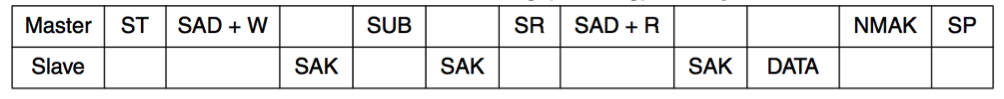
\includegraphics[width=1\textwidth]{kapitler/billeder/i2c-onebyte.png}
    \caption{SKRIV TEKST HER}
    \label{fig:i2conebyte}
\end{figure}

Figur \ref{fig:i2conebyte} viser skridt for skridt, hvordan kommunikationsprotokollen er opbygget, hvis man vil læse data én gang fra én af vores to digital komponenter.

Protokollen indeholder følgende instruktioner for at modtage én data byte:

\begin{enumerate}
\item ST (”Start Bit”): Master sender et start bit til alle slaverne, for at starte kommunikationen.
\item SAD+W (”Slave Adress + Write”): Master sender en slave adresse på 7 bits, samt ét write bit. Adressen er specifik for hver komponent og fortæller hvilken slave, som resten af kommunikationen kommer til at foregå med. Det sidste bit indikere, at masteren vil skrive noget til slaven.
\item SAK (”Slave Acknowledge”): Slaven med den valgte adresse sender er ACK bit tilbage, som fortæller at den har hørt hvad masteren sagde, og gør klar til at læse næste instruktions.
\item SUB (”Sub adress”): Master sender herefter en underadresse. Denne underadresse er en 7 bit adresse, som fortæller hvilken register inde i den valgte komponent, der gerne vil adresseres.
\item SAK (”Slave Acknowledge”): Slaven sender endnu et SAK bit, og gør klar til næste instruktion.
\item SR (”Repeated Start”): Master sender herefter et gentagende start bit. Der skal altid sendes en start/repeated start instruktion, hver gang der skiftes mellem at læse eller skrive. Ved repeated start vedholdes forbindelsen til slaven, og slaven ved derfor allerede hvilken underadresse, der herefter skal læses fra.
\item SAD+R (”Slave Adresse + Read”): Master sender herefter igen slave adressen, samt én read bit, for at ændre at vi nu gerne vil læse på slaven, modsat at vores tidligere write, som skrev til slaven.
\item SAK (”Slave Acknowledge”):  Slaven sender en ACK bit.
\item DATA (”Data Byte”): Slaven sender efterfølgende en data byte til master.
\item NMAK (”Master Not Acknowledge”): Herefter sendes én NMAK fra master til slaven, for at indikere at der ikke skal læses mere data.
\item SP (”Stop Bit”): Til sidst sender master et stop bit, for at afslutte kommunikationen.
\end{enumerate}
